\section{Boolean Retrieval} \label{ch2}
In this chapter we begin with a very simple example of an information retrieval problem, and introduce the idea of a term-document matrix and the central inverted index data structure. We will then examine the Boolean retrieval model and how Boolean queries are processed. 

\subsection{An example of IR problem}
Suppose that we want to determine which plays of Shakespeare contain the words \textit{Brutus} AND \textit{Caesar} AND NOT \textit{Calpurnia}. 

The simplest solution to this problem is grepping through the text, which can be a very effective process, especially given the speed of modern computers, and often allows useful possibilities for wildcard pattern matching through the use of regular expressions. However, this solution has some disadvantages:

\begin{itemize}
    \item it is slow, because it requires a linear scan of the entire collection of documents. This problem can be avoided exploiting an index;
    \item it does not allow to implement other operations, for example "find the word \textit{Romans} near \textit{countrymen}";
    \item we would like to have a ranked retrieval, i.e. to return the best documents according to the user's information need.
\end{itemize}

Two important operations in IR are \textbf{tokenization} and \textbf{vectorization}. Tokenization's goal is to segment a text into words or characters, while vectorization is the process of transforming text into numeric vectors.
Suppose we record for each document whether it contains each word out of all the words Shakespeare used (Shakespeare used about 32,000 different words): the result is a binary \textbf{term-document incidence matrix}, as represented in Picture \ref{inc_mat}.

\begin{figure}[h!]
		\centering
		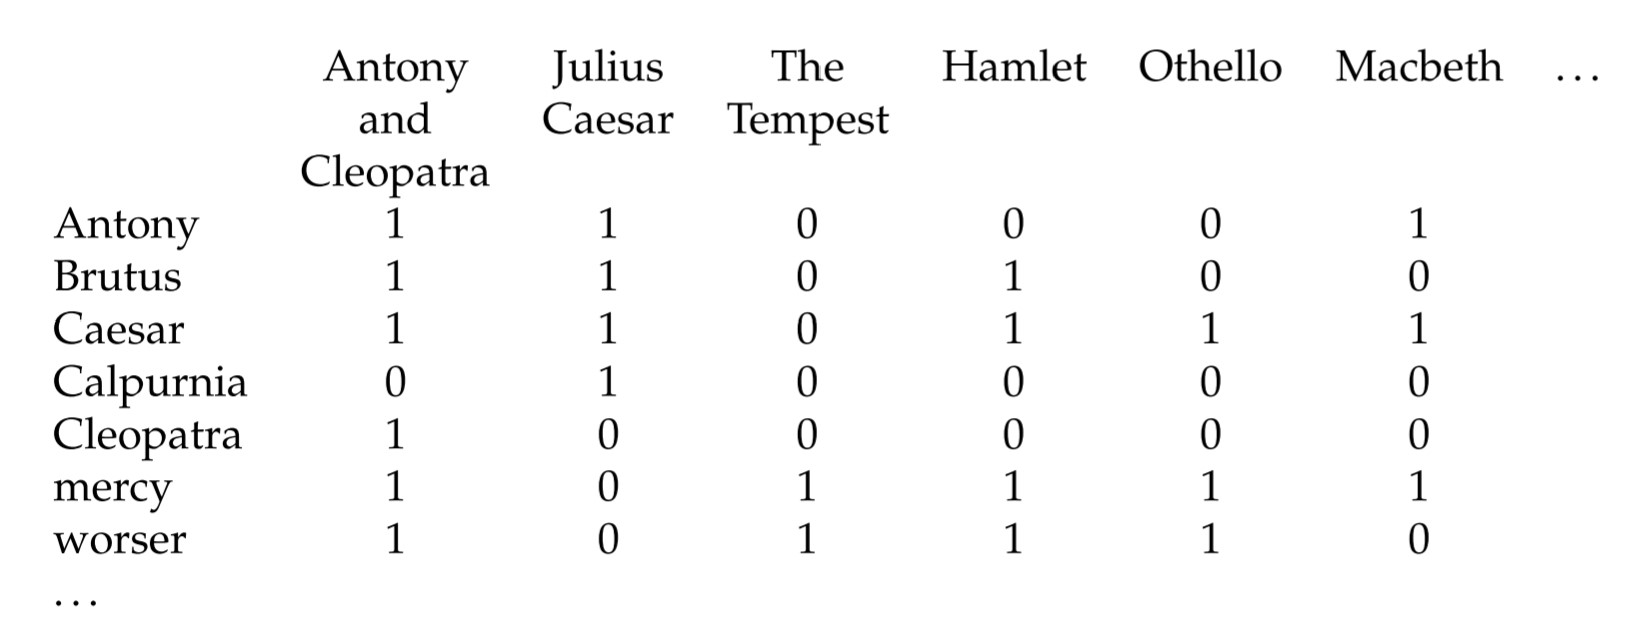
\includegraphics[scale = 0.6]{img/incidence matrix.jpg}
		\label{inc_mat}
\end{figure}

In this matrix, for each term we have a binary vector representing the set of documents including the term. Using this representation, we can answer the previous query by computing a bitwise AND between the vectors of \textit{Brutus}, \textit{Caesar} and \textit{Calpurnia} (complemented). The result is: 110100 AND 110111 AND 101111 = 100100, i.e. the plays that satisfy the query are \textit{Antony and Cleopatra} and \textit{Hamlet}.

In this sense, a \textbf{Boolean retrieval model} is a model for information retrieval in which we can pose any query which is in the form of a Boolean expression of terms, that is, in which terms are combined with the operators AND, OR, and NOT. In this model each document is represented by just using a set of words.

Let's consider a more realistic scenario, and suppose that we have a collection composed of $N = 1$ million documents, each of which is in turn composed of 1000 words (so 1G words in total). If we assume an average of 6 bytes per word, then the size of the collection is 6GB, and if there are $M = 500K$ distinct terms among the collection, then the matrix would have a dimension 500K x 1M. Moreover, since the collection only contains 1G of words, the matrix would be extremely sparse. For this reason, the matrix representation is not feasible for real world data dimension, so a much better representation is given by storing for each term only the documents in which that term appears. This approach can be implemented using the inverted index.

\subsection{Inverted Index}
As introduced before, the idea of the \textbf{inverted index} structure is that for each term $t$, we only store a list of all the documents that contain $t$, the so called postings list. 

\begin{figure}[h!]
		\centering
		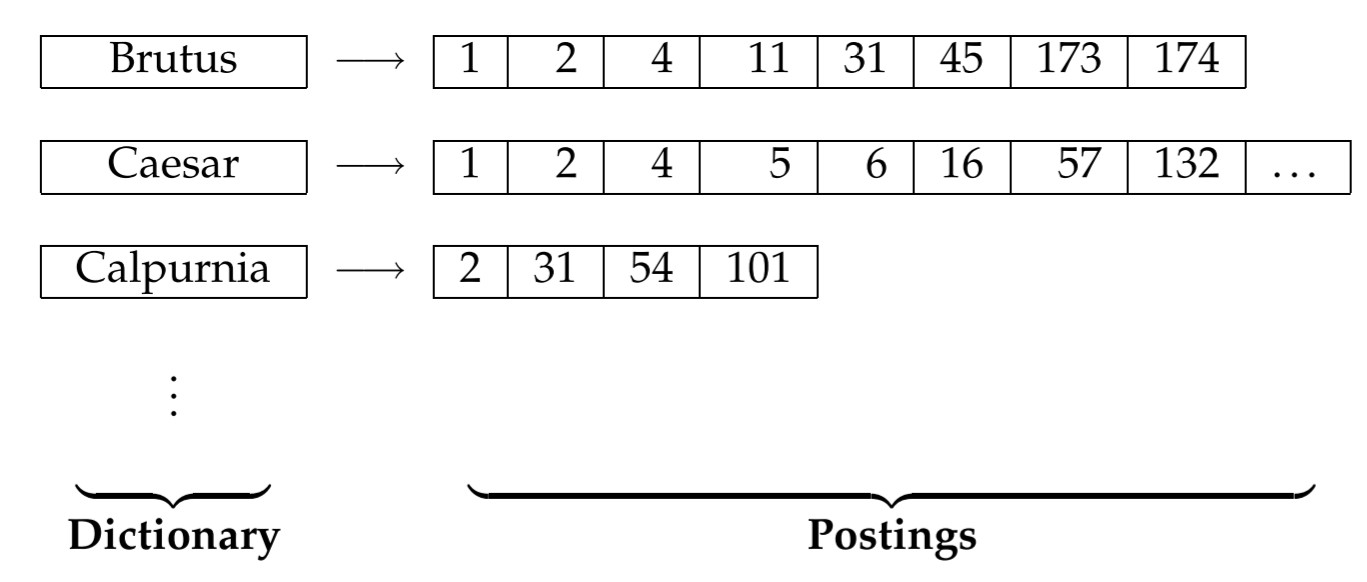
\includegraphics[scale = 0.6]{img/inverted index.jpg}
		\label{inc_mat}
\end{figure}

Usually, the dictionary is stored in the memory, with pointers to each postings list, which is stored on disk. The inverted index construction follows the following steps:

\begin{enumerate}
    \item Collect the documents to be indexed;
    \item Tokenize the text, turning each document to a list of tokens;
    \item Apply some linguistic preprocessing in order to obtain the indexing terms (ex: stemming, removing stop words, etc..);
    \item Create the inverted index combining dictionary and postings.
\end{enumerate}

An example of this building process in represented in Picture \ref{inc_ex}

\begin{figure}[h!]
		\centering
		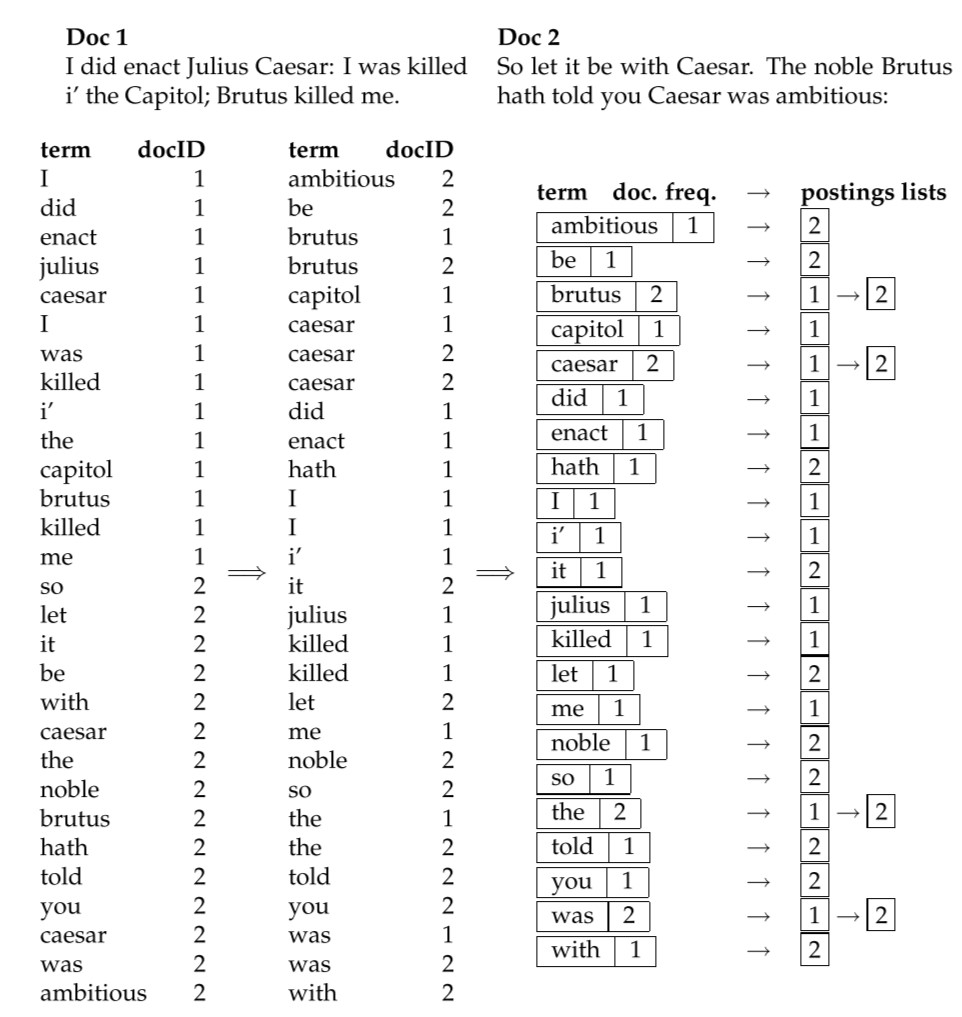
\includegraphics[scale = 0.8]{img/example_inverted index.jpg}
		\label{inc_ex}
\end{figure}

As we can see in the example, the terms of the dictionary are sorted in alphabetical order, and for each term the document frequency information, i.e. the length of its postings list, is added for each term, and it can be helpful for improving the efficiency of the search engine at query time. Since both the dictionary and the postings list are stored, their size is important. Concerning the postings list, a fixed length array would be wasteful as some words occur in many documents, and others in very few, so two good alternatives are \textbf{singly linked lists} or \textbf{variable length arrays}. However, variable length arrays win in space requirements by avoiding the overhead for pointers and in time requirements because their use of contiguous memory increases speed on modern processors with memory caches.

\subsection{Processing boolean queries}
Now the question is: how do we process a query using the inverted index structure and the boolean retrieval model? In we consider the query "\textit{Brutus} AND \textit{Caesar}", then the result can be obtained with the following steps:

\begin{enumerate}
    \item locate \textit{Brutus} in the dictionary;
    \item locate \textit{Caesar} in the dictionary;
    \item compute the intersection of the two postings lists;
\end{enumerate}

\begin{figure}[h!]
		\centering
		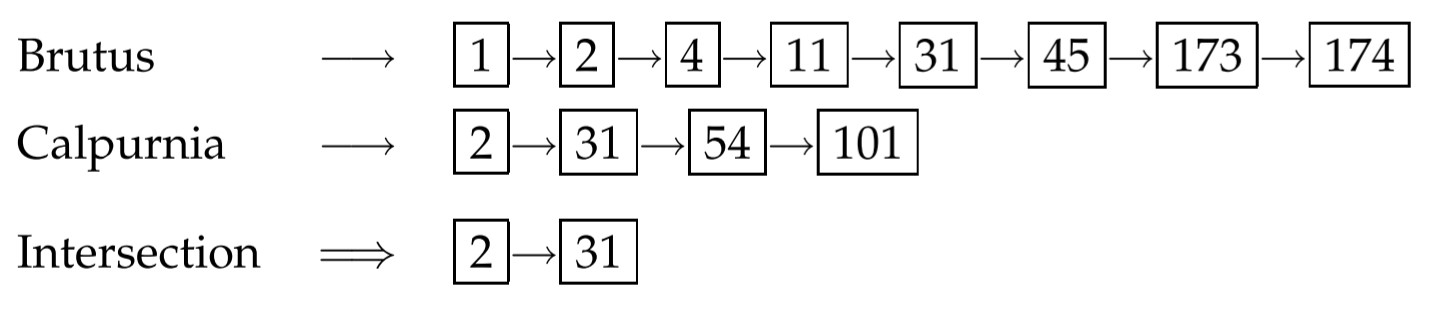
\includegraphics[scale = 0.8]{img/boolean query_inv.jpg}
		\label{inc_ex}
\end{figure}

As we can imagine, the intersection (or merging) operation is crucial: it must be able to retrieve in a fast way the documents that contain both terms. A possible implementation of the intersection operation is represented in Picture \ref{intersection}: in this case the complexity of the operation is $O(x + y)$, where $x$ and $y$ are the lengths of the two postings lists. Note that a crucial assumption of this implementation is that the two lists are sorted.

\begin{figure}[h!]
		\centering
		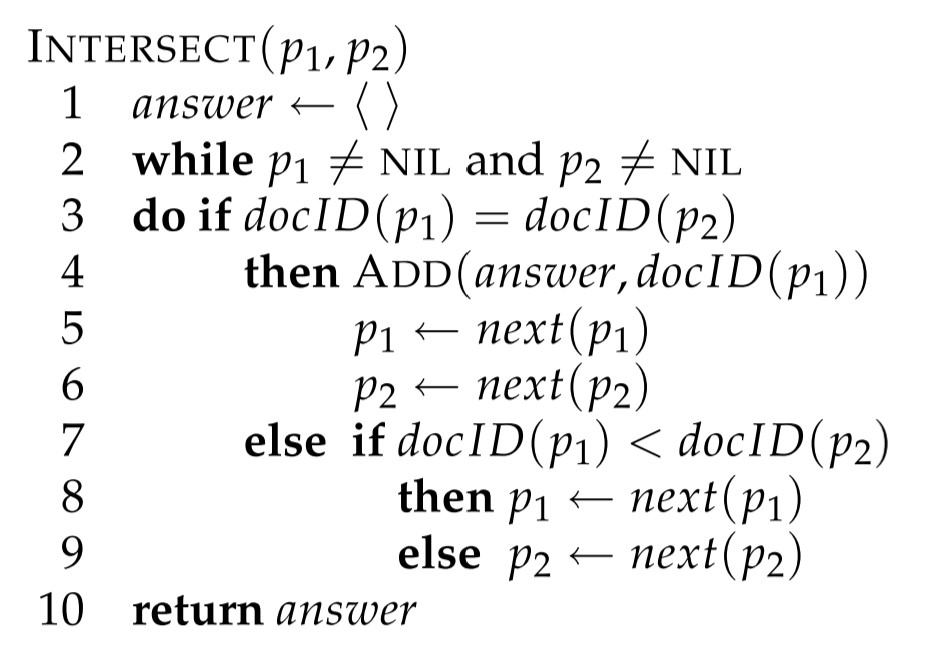
\includegraphics[scale = 0.8]{img/intersection.jpg}
		\label{intersection}
        \caption{Basic implementation of the intersection operation}
\end{figure}

One possible way to speedup the intersection operation is represented by the usage of the \textit{postings list with skip pointers} data structure, as shown in Picture \ref{postings with skip}. Skip pointers are effectively shortcuts that allow us to avoid processing parts of the postings list that will not figure in the search results: at each position of the postings list we can either process the following element or use the pointer to skip irrelevant elements. 

\begin{figure}[h!]
		\centering
		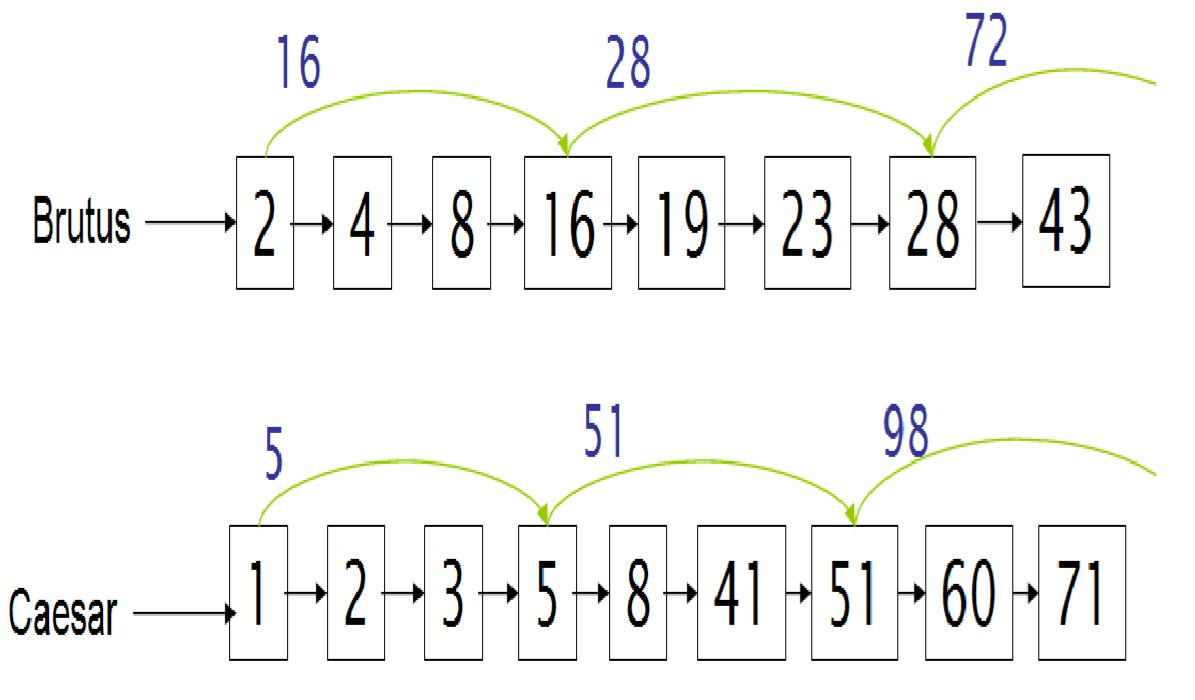
\includegraphics[scale = 0.5]{img/postings with skip.jpg}
		\label{postings with skip}
        \caption{Postings list with skip pointers}
\end{figure}

Now the two questions are \textbf{where} to place skip pointers and \textbf{how} to do efficient merging using skip pointers. Suppose we're considering the two postings lists of Picture \ref{postings with skip}, and that we have matched 8 on each list: we advance both pointers and we reach 16 in the first list, and 41 in the second. Now, since the skip list pointer points to 28, which is still less than 41, we can exploit it to jump directly to 28, without processing 19, and 23. Notice that this is possible thanks to the assumption that the lists are sorted. An example of \textbf{algorithm} that implements the merge operation using the postings lists with skip pointers is shown in Picture \ref{posting intersection with skip}.

\begin{figure}[h!]
		\centering
		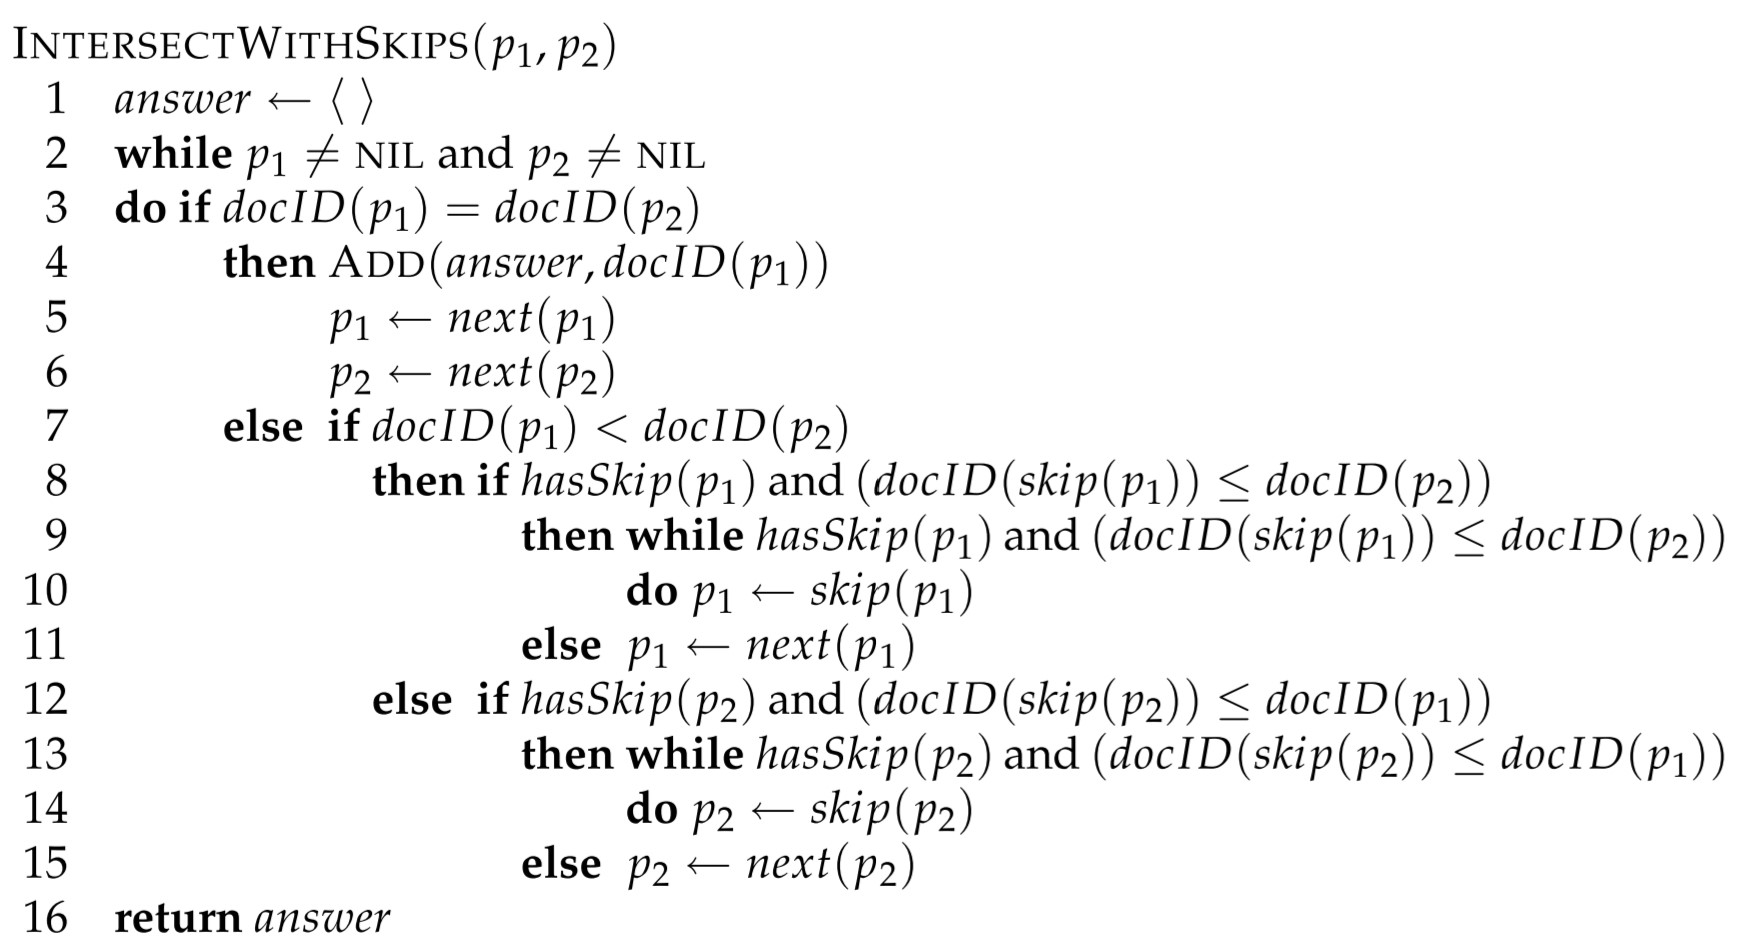
\includegraphics[scale = 0.6]{img/posting intersection with skip.jpg}
		\label{posting intersection with skip}
        \caption{Postings lists intersection with skip pointers}
\end{figure}

Regarding the \textbf{place} in which inserting the skip pointers, there's a \textbf{trade-off} between the number of pointers and the space that they occupy. On the one hand, the more skip pointers, the shorter the skip spans will be, resulting in many comparisons to skip pointers and a lot of space used to store them. On the other hand, the fewer skip pointers, the longer the skip spans will be, resulting in less opportunities to skip and, consequently, in less successful skips. A simple \textbf{heuristic} indicates that for postings list of length $P$ we should use $\sqrt{P}$ evenly-spaced skip pointers, ignoring the distribution of query terms.

In general, building effective skip pointers is easy if an index is relatively static, but it is harder if a postings list keeps changing because of updates.

\subsection{Properties}
Among the advantages, we underline:

\begin{itemize}
    \item It is \textbf{precise}, if the right strategies for searching are known;
    \item It is \textbf{efficient} for computers.
\end{itemize}

On the other hand, the disadvantages are:

\begin{itemize}
    \item The user must learn the \textbf{boolean logic};
    \item The \textbf{boolean logic} is \textbf{insufficient} to capture the \textbf{richness of the language};
    \item There's \textbf{no control} over the \textbf{size of the result set}: either too many or none documents are returned. Moreover, \textbf{all} the documents in the results are considered \textbf{equally good}, i.e. there's no rank for the documents in the solution;
    \item It \textbf{does not support partial matches}.
\end{itemize}

\subsection{Query optimization}
An important issue about \textit{Boolean retrieval model} is represented by understanding which is the best order for query processing. Suppose we're dealing with the following query \textit{Brutus} AND \textit{Calpurnia} AND \textit{Caesar}: for each term we have to get their postings and AND them together. In this case, the best choice would be to process the postings in order of increasing frequency, i.e. start with the smallest postings, by exploiting the document frequency information which is stored. By following this approach, the \textit{intersect} operation is implemented as shown in Picture \ref{sort_intersect}.

\begin{figure}[h!]
		\centering
		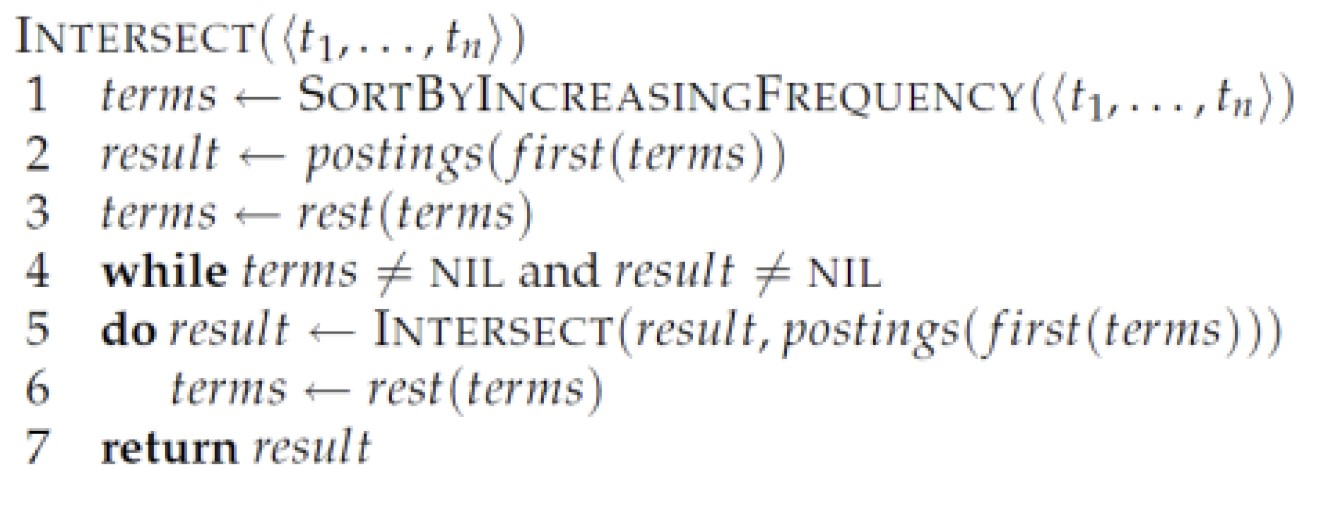
\includegraphics[scale = 0.6]{img/sort_intersect.jpg}
		\label{sort_intersect}
\end{figure}

If we consider another query, for example (\textit{Brutus} OR \textit{Caesar}) AND NOT (\textit{Anthony} OR \textit{Cleopatra}) AND (\textit{Brutus} OR \textit{Cleopatra}), then another approach to speedup the query could be estimate the size of each OR operation by the sum of its document frequencies, and then process in increasing order of the OR sizes.

\subsection{Positional postings and phrase queries}
Most recent search engines support a double quotes syntax (\textit{“stanford university”}) for \textbf{phrase queries}, which has proven to be very easily understood and successfully used by users, as 10\% of web queries are phrase queries, and many more are implicit phrase queries (such as person names), entered without use of double quotes. 

To be able to support such queries, it is no longer sufficient for postings lists to be simply lists of documents that contain individual terms. In this section we consider three approaches to supporting phrase queries and their combination in an efficient way.

\subsubsection{Biword indexes}
One approach could be considering each pair of consecutive terms (biword) in a document as a phrase: for example, the text \textit{"Friends, Romans, Countrymen"} would generate two biwords: \textit{"friends romans"} and \textit{"romans countrymen"}. Each of the \textbf{biword} is now a \textbf{dictionary term}, so in this particular case we would be able to solve a two-word phrase query processing in an immediate way. In general, longer queries can be processed by breaking them down: for example the query \textit{"stanford university palo alto"} can be broken into the following boolean query on biwords: \textit{"stanford university"} AND \textit{"university palo"} AND \textit{"palo alto"}. 

Two important issues about biwords are:

\begin{itemize}
    \item There can be some \textbf{false positives}: without examining the documents, we cannot verify that the documents matching the Boolean query do actually contain the original word phrase;
    \item The problem of the \textbf{index blowup} due to bigger dictionaries.
\end{itemize}

For these reasons, the biword index is not the standard solution, but it can be part of a compound strategy.

\subsubsection{Positional indexes}
This approach is most commonly employed, and it is based on the idea of storing, for each term in the vocabulary, the postings of the form docID: <position1, position2, .., >, where each position is a token index in the document. Each posting will also usually record the term frequency. An example of positional index is provided in Picture \ref{pos_index}: as we can see, for each term, the term frequency is indicated, along with the term frequencies and the positions for each document. In this case, \textit{to} has a document frequency of 993,427, and it appears 6 times in document 1 at positions 7, 18, etc..

\begin{figure}[h!]
		\centering
		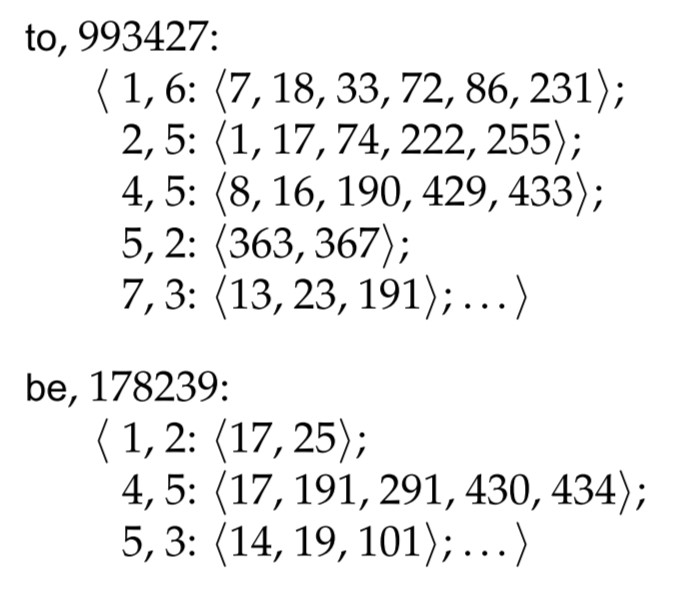
\includegraphics[scale = 0.8]{img/positional_index.jpg}
		\label{pos_index}
        \caption{Positional index}
\end{figure}

To process a phrase query, we still need to access the inverted index entries for each distinct term. As before, we would start with the least frequent term and then work to further restrict the list of possible candidates. In the \textbf{merge operation}, the same general technique is used as before, but rather than simply checking that both terms are in a document, we also need to \textbf{check} that \textbf{their positions} of appearance in the document are compatible with the phrase query being evaluated. This requires working out offsets between the words. For example, suppose that the positional index for the words \textit{to} and \textit{be} are the ones in Picture \ref{pos_index}, and that the query is \textit{to be or not to be}  in this case we first look for the documents that contain both terms, in this case doc1, doc4 and doc5. Then, we look for places in the lists where there is an occurrence of \textit{be} with a token index one higher than a position of \textit{to}, and then we look for another occurrence of each word with token index 4 higher than
the first occurrence. In the above list, these conditions are guaranteed for doc4, since \textit{to} appears in positions 429 and 433, while \textit{be} appears in positions 430 and 434. Notice that doc4 represents a good candidate for solving the query, but an additional check must be performed for terms \textit{or} and \textit{not}.

In general, positional indexes allow to solve $k$ word proximity searches, i.e. searches in which we fix a windows, while biword indexes cannot. Picture \ref{pos_intersect} shows an algorithm for implementing the $k$ word proximity searches: the algorithm finds places where the two terms appear within $k$ words of each other and returns a list of triples giving docID and the term position in $p1$ and $p2$.

\begin{figure}[h!]
		\centering
		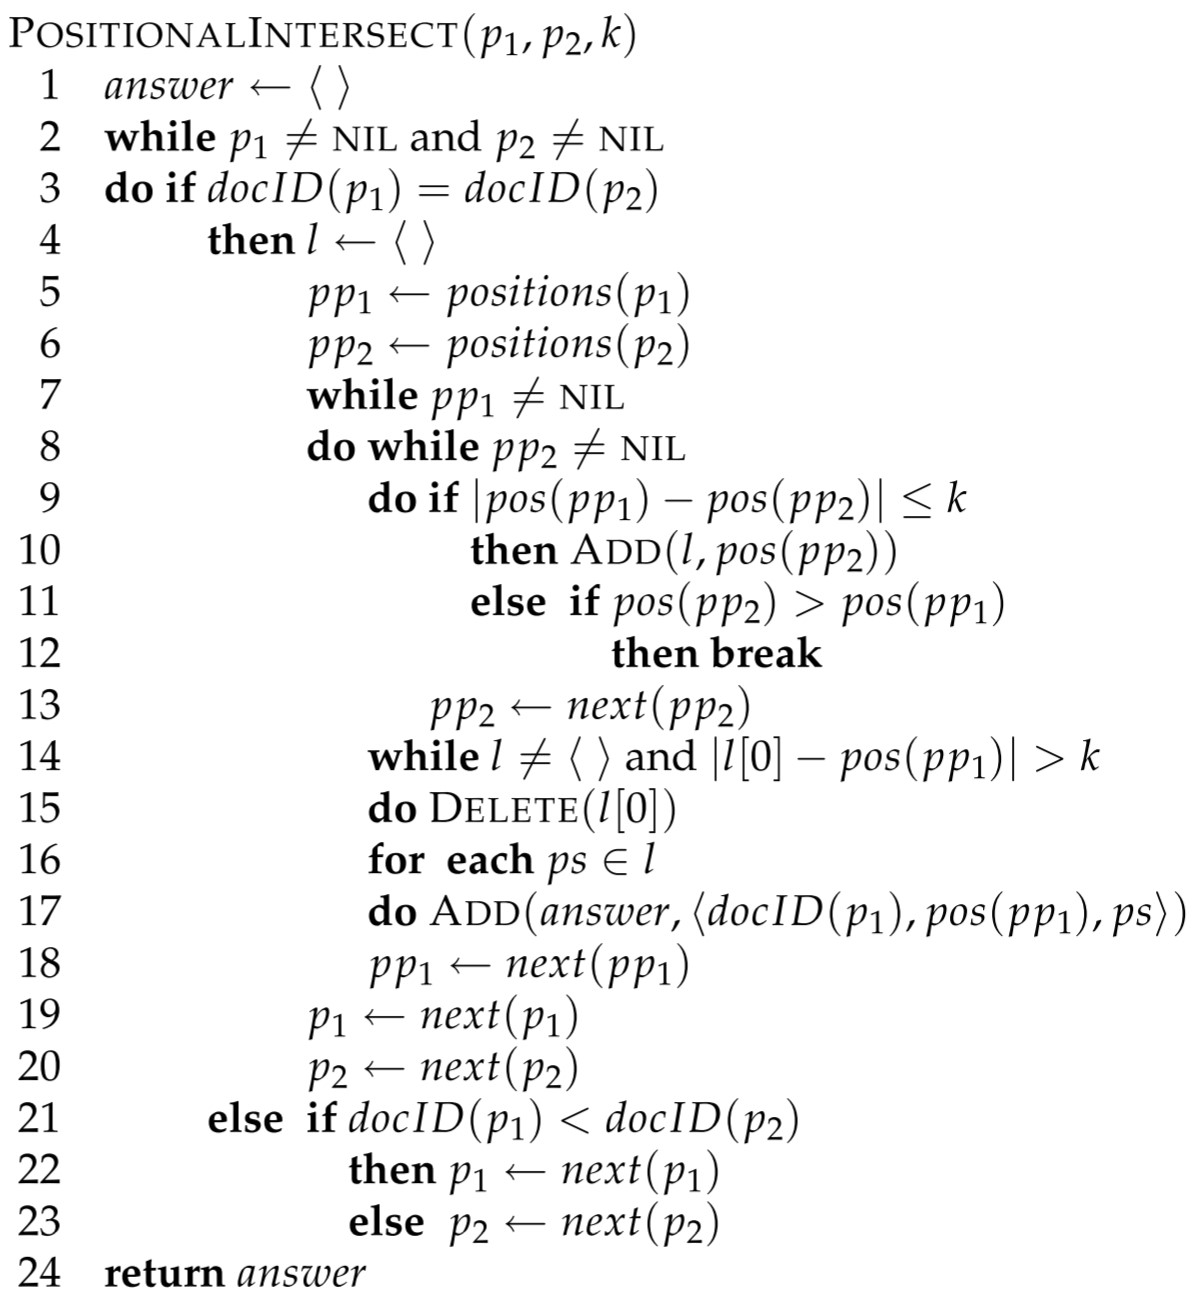
\includegraphics[scale = 0.8]{img/positional_intersect.jpg}
		\label{pos_intersect}
        \caption{Algorithm for proximity intersection of two postings lists}
\end{figure}

A positional index \textbf{expands postings storage substantially}, even if the positions/offsets are compressed. Indeed, the asymptotic complexity of a postings intersection operation is no longer bounded by the number of documents $N$, but by the total number of tokens in the document collection $T$. However, positional indexes are now \textbf{standardly used}, because of the power and usefulness of phrase and proximity queries. From the point of view of space implication, since a posting needs an entry for each occurrence, the \textbf{index size} depends on the \textbf{average document size}: the average web page has less than 1000 terms, but financial documents, books etc.. may easily reach 100,000 terms. If we consider an average term frequency of 0.1\%, then large documents cause an increase of two orders of magnitude in the space required to store the postings list, as represented in Picture \ref{space_pos_index}.

\begin{figure}[h!]
		\centering
		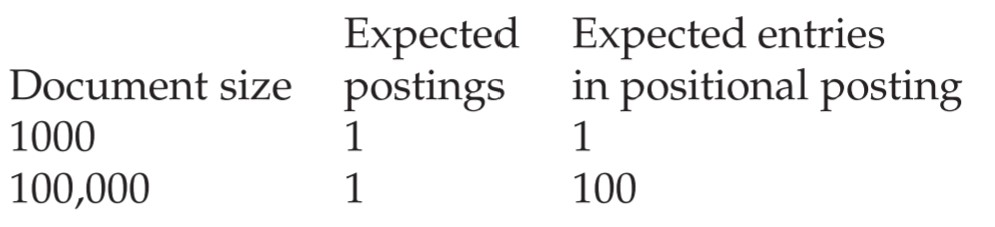
\includegraphics[scale = 0.8]{img/space positional indexes.jpg}
		\label{space_pos_index}
        \caption{Average number of positional postings with different document sizes}
\end{figure}

In general, according to some rules of thumb, a positional index is 2 to 4 times as large as a non-positional index, and a compressed positional index is about one third to one half the size of the raw text (after removal of markup, etc.) of the original uncompressed documents.

\subsubsection{Combination schemes}
This strategy combines the biword and the positional indexes approach, since it uses a phrase index, or just a biword index, for certain queries and uses a positional index for other phrase queries. The idea behind this approach is that it is usually inefficient to keep on merging positional postings lists, so for this reason the most common queries are included in the phrase index. Williams et al. (2004) evaluated a more sophisticated mixed indexing scheme, composed of biwords and positional indexes, and a typical web query mixture was executed in one-fourth of the time of using just a positional index. However, it required 26\% more space than having a positional index alone.

